\newpage

\section*{ $^{63}$Cu(n,$\gamma$)$^{63}$Cu }

Power Level: 100 kW(th) \\
Time at Power: 3600 s \\
Wait Time: 172800 s \\
Total Activity at Removal: 3.94e+01 $\mu Ci$

\begin{table*}[h]
\centering
\begin{tabular}{ |c|c|c|c|c|c| }
 \hline
 Position & Mass $mg$ & Counting Time $s$ & Counting Activity $\mu Ci$ & Expected Area (Counts) \\
 \hline 
 1 & 1.348290013679891 & 3600 & 4.87e+00 & 4.74e+04\\ 
\hline
 2 & 1.348290013679891 & 3600 & 7.37e+00 & 7.17e+04\\ 
\hline
 3 & 1.348290013679891 & 3600 & 6.78e+00 & 6.59e+04\\ 
\hline
 4 & 1.348290013679891 & 3600 & 3.88e+00 & 3.77e+04\\ 
\hline
\end{tabular}
\end{table*}

\begin{figure}[!ht]
   \centering
   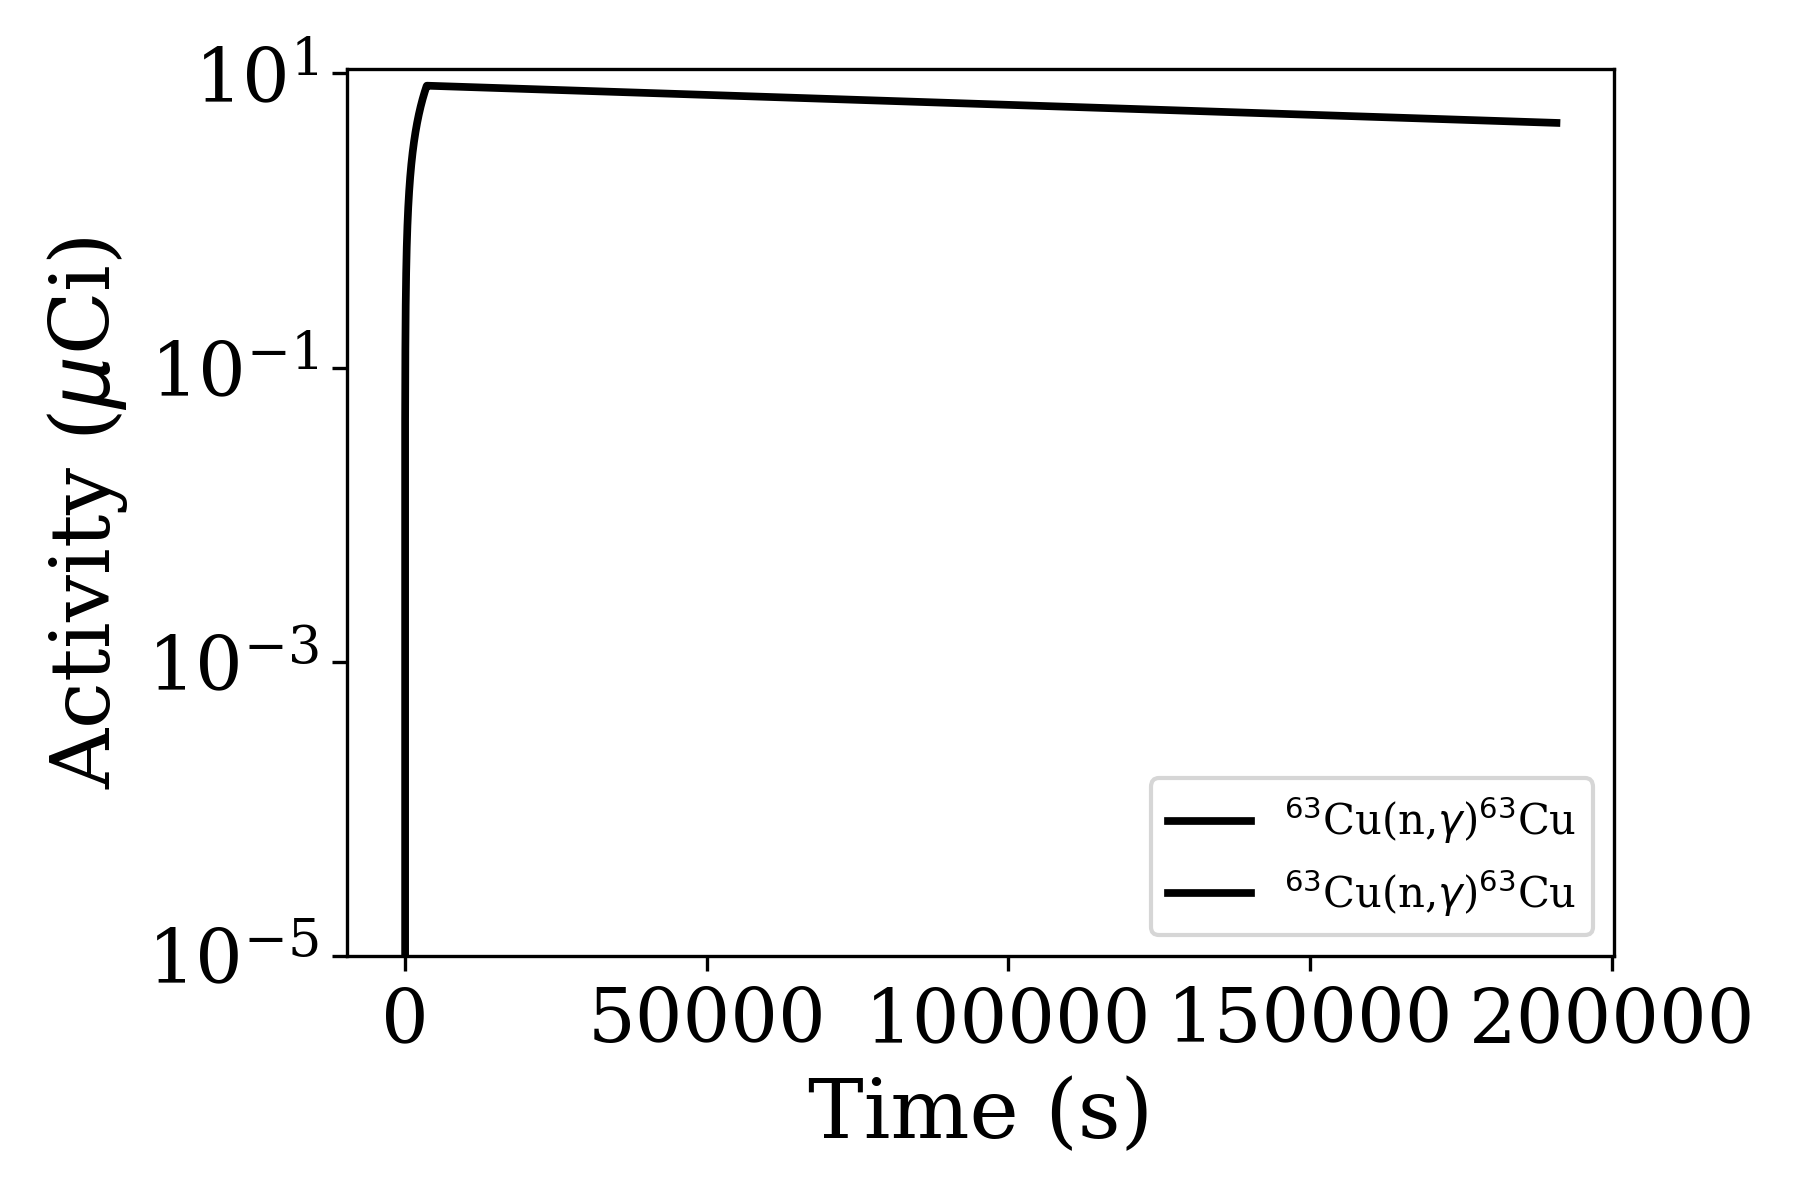
\includegraphics[width=.4\textwidth]{source/plot/Cu-63(n,gamma)Cu-64_wisconsin1.png} 

\end{figure}

\begin{figure}[!ht]
   \centering
   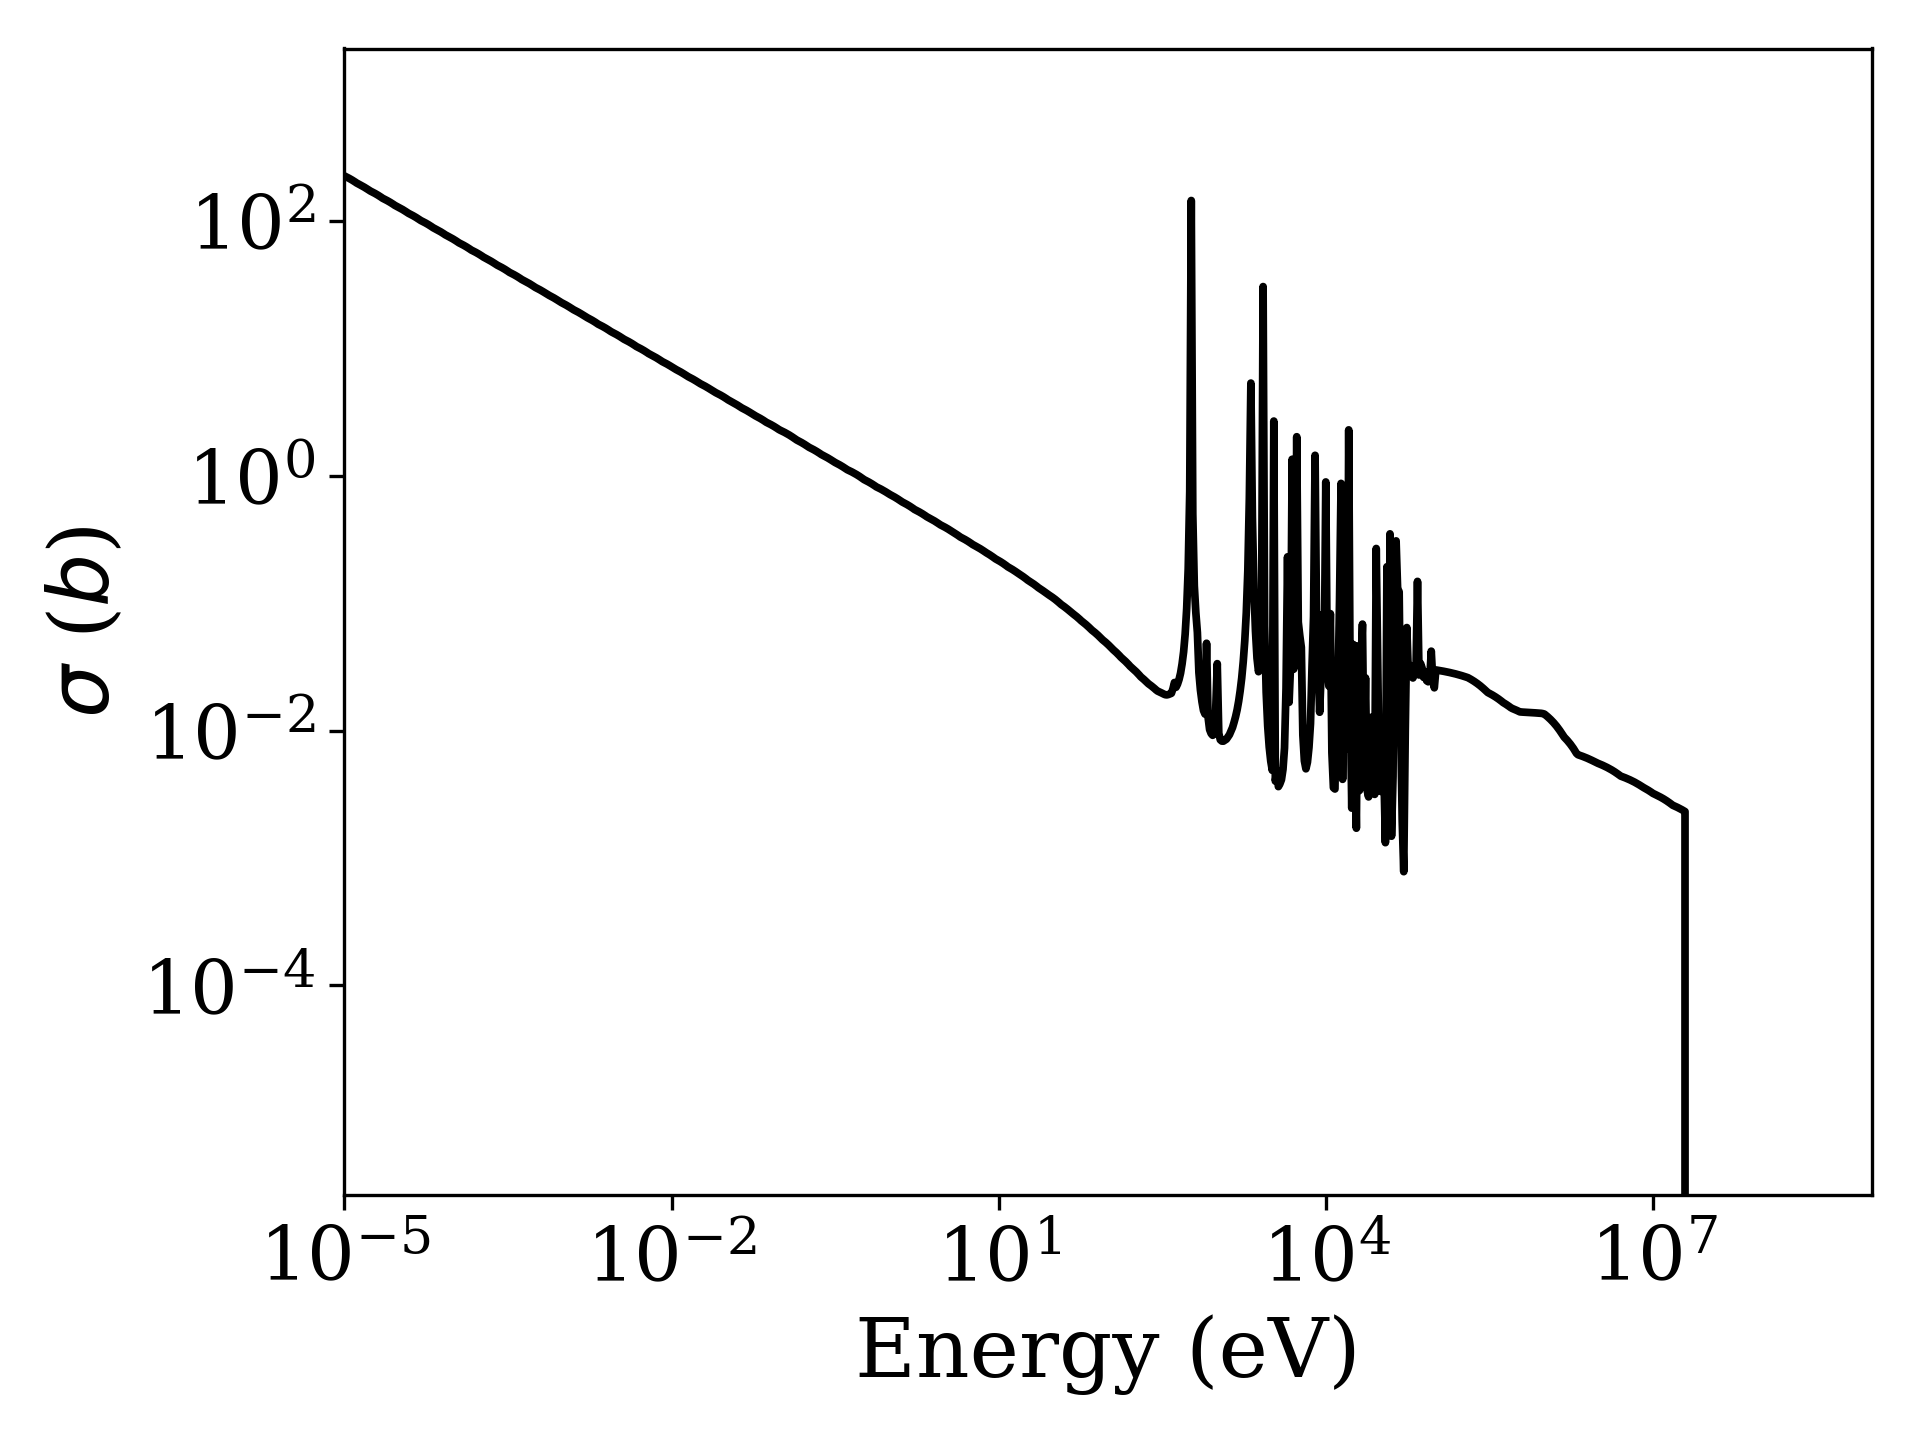
\includegraphics[width=.4\textwidth]{source/plot/Cu-63(n,gamma)Cu-64.png} 

\end{figure}

\begin{table*}[h]
\centering
\begin{tabular}{ |c|c|c|c|c|c|c| }
 \hline
 Reaction & T$_{1/2}$ & ROI (eV) & Important Gammas (keV) \\
 \hline 
 $^{63}$Cu(n,$\gamma$)$^{63}$Cu &  2.6 d & 7.01e-03, 5.79e+02 & 1345.77(0.00475),  \\ 
\hline
\end{tabular}
\end{table*}
